\section{Software-Verzeichnisse und Paketverwaltung}
\label{sec:paketverwaltung}
Im Gegensatz zur Versionsverwaltung verwaltet die Paketverwaltung keinen Code und dessen Änderungen, sondern fertige Softwarepakete, welche von Entwicklern erstellt und in einem Software-Verzeichnis abgelegt werden.
Inhalt eines Pakets können standardisierter Code von Software-Modulen oder kompilierter Code sein.
Zusätzlich werden in einem Paket Metadaten gespeichert.
Diese Metadaten können eine Beschreibung, Version, Abhängigkeiten und Autoren des Pakets enthalten.
Sie lassen sich aus dem Paket mithilfe des Paketverwaltungssystems auslesen oder über APIs des Software-Verzeichnisses abrufen.
Außerdem übernimmt das Paketverwaltungssystem das Installieren und meistens auch das Aktualisieren und Deinstallieren von Paketen.
Zusätzlich wird das System verwendet, um fehlende Abhängigkeiten von Paketen automatisch zu installieren \autocite{spinellis_package_2012}.

In dieser Arbeit wird auf die Software-Verzeichnisse \gls{pypi} und \gls{cran} eingegangen.
\gls{pypi} ist das Verzeichnis für Python-Pakete und \gls{cran} ist das Verzeichnis für R-Pakete.
In \gls{pypi} sind aktuell mehr als 500.000 unterschiedliche Projekte mit über 5 Millionen Veröffentlichungen verfügbar \autocite{python_software_foundation_pypi_2024}.
\gls{cran} listet aktuell mehr als 20.000 Pakete \autocite{cran_team_comprehensive_2024}.

\subsection{PyPI}
\label{subsec:paketverwaltung_pypi}
\gls{pypi} hat zu Beginn des Jahres 2024 ein \gls{pep} veröffentlicht, welches die Verifizierung von Daten auf \gls{pypi} beschreibt \autocite{python_software_foundation_pep_2024}.
In dem \gls{pep} werden Änderungen an der API beschrieben, welche zum Hochladen von Paketen genutzt wird, um sogenannte \glqq Attestation objects\grqq{} zu unterstützen, in denen digitale Signaturen enthalten sind.
Das Ziel ist es verifizierte Daten auf \gls{pypi} zu ermöglichen, sodass Anwender direkt erkennen können, ob die Daten vertrauenswürdig sind.
Aktuell wird dieses \gls{pep} umgesetzt, wodurch es zu vielen Änderungen in der API und auch in der Weboberfläche von \gls{pypi} kommt.

Außerdem sind noch nicht alle Daten über die APIs erreichbar und es ist auch aktuell nicht über die API erkennbar, ob es sich um verifizierte oder nicht verifizierte Daten handelt.
Ein Beispiel für verifizierte Daten sind Links, beispielsweise zu GitHub.
Diese Links werden von \gls{pypi} als verifiziert angesehen, wenn der Upload des Pakets auf \gls{pypi} über eine GitHub-Action erfolgt.
Zudem werden die Personen als verifiziert dargestellt, welche in \gls{pypi} als Owner oder Betreuer des Pakets eingetragen sind, sie haben somit einen Account bei \gls{pypi}.
Der dargestellte Owner kann nicht über eine API abgefragt werden.

\begin{figure}
    \begin{center}
        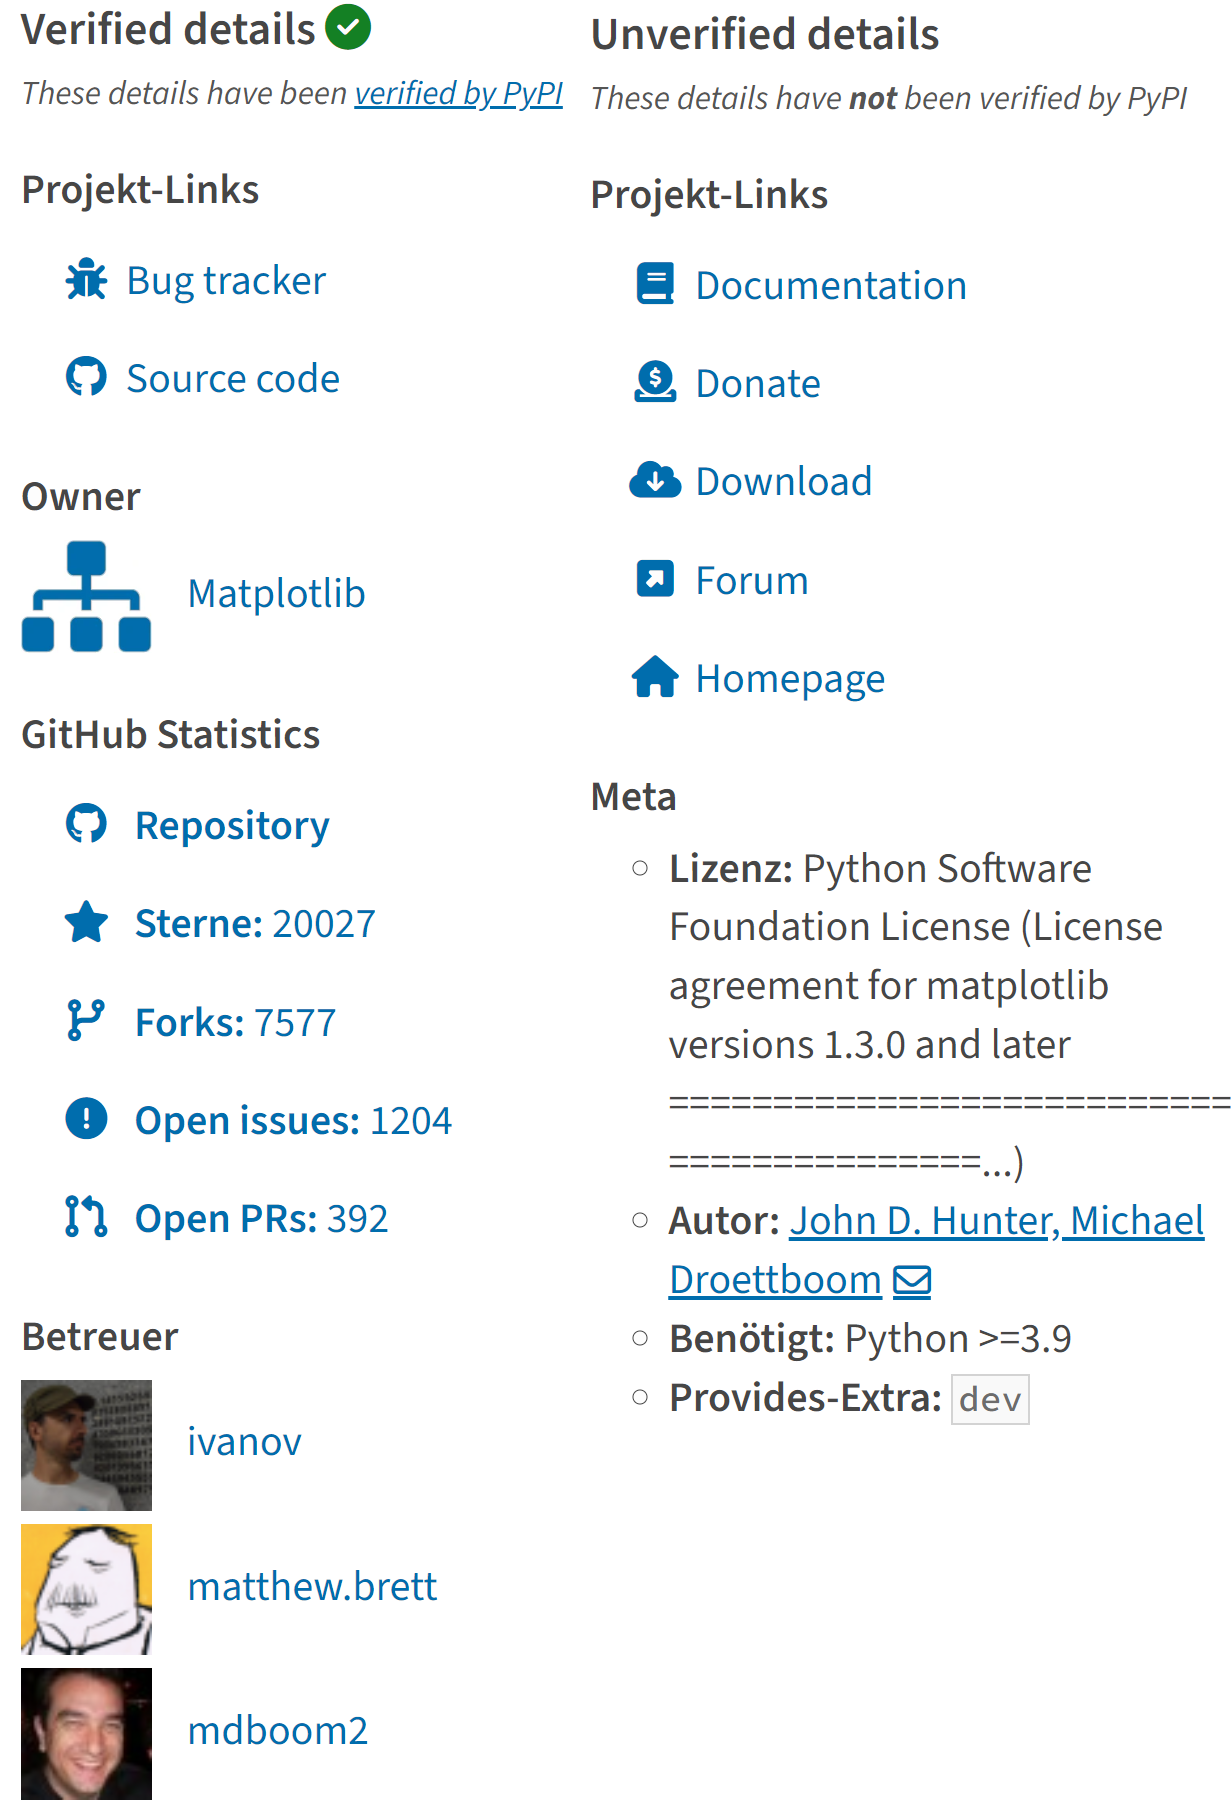
\includegraphics[width=0.95\textwidth]{bilder/pypi.png}
    \end{center}
    \caption{\gls{pypi} Verifizierte und unverifizierte Daten}
    \label{fig:pypi_verified_unverified_details}
    \small
    Die Abbildung stellt die verifizierten und unverifizierten Daten des Pakets \emph{matplotlib} auf \gls{pypi} dar \autocite{python_software_foundation_pypi_2024}.
\end{figure}

\gls{pypi} bietet verschiedene APIs und Quellen an, um die Daten der Pakete abzufragen.
Im Folgenden werden auf einige der Zugriffsmöglichkeiten eingegangen, welche mit Ausnahme der BigQuery alle in dieser Arbeit verwendet werden.

\subsubsection*{JSON-API}
\label{subsubsec:pypi_json_api}
% TODO ggf. die nicht verifizierten Daten stammen aus der Python toml (stammen die Daten wirklich alle aus der toml?) Falls ja das erwähnen und erklären, dass die Daten direkt von dem Python-Paket stammen und pypi diese nur durchreicht
Die JSON-API ist die bevorzugt zu verwendende API von \gls{pypi} und bietet die Möglichkeit, die Metadaten eines Pakets abzufragen \autocite{python_software_foundation_warehouse_2024}.
Diese API ist nicht in der Anzahl der Anfragen beschränkt.
Daten der neuesten Version des Pakets werden von der API zurückgegeben.
Die Werte in den Metadaten stammen aus den Daten, welche beim Hochladen auf \gls{pypi} angegeben wurden.
Die Daten des ersten Uploads eines Releases werden dabei als Metadaten der Version gespeichert und bei weiteren Uploads dieser Version nicht überschrieben.

Inhalt der Metadaten sind beispielsweise die Autoren und Maintainer zuzüglich deren E-Mail-Adresse, die Beschreibung, Lizenz und Links zu unterschiedlichen Quellen, beispielsweise einem GitHub-Repository \autocite{python_software_foundation_warehouse_2024}.
Die Beschreibung kann den Text aus der README-Datei des Pakets auf GitHub enthalten.
Es ist jedoch auch möglich, eine eigene Beschreibung für \gls{pypi} anzugeben, sodass sich die README-Datei in GitHub und die Beschreibung auf \gls{pypi} unterscheiden können.
Die Metadaten werden von den Entwicklern des Pakets eingetragen.
In \autoref{fig:pypi_verified_unverified_details} sind einige der Metadaten des Pakets \emph{matplotlib} unter dem Punkt \glqq Meta\grqq{} dargestellt.
Weitere Daten sind unter dem Punkt \glqq Projekt-Links\grqq{} unter den verifizierten Details dargestellt.

Die Autoren und Maintainer aus den Metadaten müssen nicht den verifizierten Betreuern und Owner des Pakets auf \gls{pypi} entsprechen, da dies unterschiedliche Systeme sind.
Zum einen sind es die Benutzer, welche Rechte auf \gls{pypi} haben, um das Paket dort anzupassen und zum anderen sind es die Personen, welche durch die Entwickler des Pakets angegeben werden.
Die Autoren und Maintainer können jedoch ebenfalls verifiziert sein, wobei dies über die API noch nicht abgefragt werden kann, jedoch in der Weboberfläche bereits für einige Pakete dargestellt wird.
Es gibt aktuell wenige Pakete, bei denen die Autoren verifiziert sind.
Ein Beispiel ist das Paket \emph{hololinked}, das Stand 28.12.2024 solche Angaben enthält \autocite{venkatasubramanian_vaidyanathan_hololinked_2024}.
\emph{Matplotlib} unterstützt dies aktuell noch nicht, wie in \autoref{fig:pypi_verified_unverified_details} dargestellt ist.
Die verifizierten Betreuer und Owner können aktuell nicht über die JSON-API abgerufen werden, sondern müssen über die XML-RPC-API abgefragt werden.

\subsubsection*{XML-RPC-API}
\label{subsubsec:pypi_xml_rpc}
Die \gls{pypi} XML-RPC-API ist eine veraltete API, welche jedoch noch genutzt werden kann, um einige Informationen zu den Paketen abzufragen.
Es wird empfohlen, diese API nicht mehr zu verwenden und den RSS-Feed oder die JSON-API als mögliche Alternativen zu verwenden \autocite{python_software_foundation_warehouse_2024}.
Außerdem ist die API in der Anzahl der möglichen Anfragen stark limitiert und auch die Abstände zwischen den Anfragen müssen groß sein.
\gls{pypi} macht keine genauen Angaben darüber, wie viele Anfragen in welchem Zeitraum möglich sind.
Diese API ist jedoch die einzige Quelle, um die Betreuer eines Pakets abzufragen, ohne einen Web-Scraper einsetzen zu müssen.
Web-Scraping bezeichnet das Extrahieren von Daten aus Webseiten, indem der HTML-Code der Webseite analysiert wird \autocite{richardson_beautifulsoup4_2024}.

Die Betreuer, welche über die API ausgegeben werden, enthalten den Benutzernamen auf \gls{pypi}, ein Vollname wird hierbei nicht ausgegeben.
Außerdem enthalten sie eine Rollenbezeichnung, welche entweder \emph{Maintainer} oder \emph{Owner} sein kann, welcher in der Oberfläche nicht dargestellt wird.
Owner können alle Änderungen am \gls{pypi} Projekt vornehmen und Betreuer können neue Versionen des Pakets veröffentlichen \autocite{ingram_deprecate_2023}.
Die Benutzernamen für die Betreuer des Pakets \emph{matplotlib} sind in \autoref{fig:pypi_verified_unverified_details} unter dem Punkt \glqq Betreuer\grqq{} dargestellt.
Aktuell stellt \gls{pypi} keine API bereit, um den Namen eines Benutzers abzufragen, sodass nur der Benutzername über eine API abgefragt werden kann \autocite{python_software_foundation_add_2024}.

\subsubsection*{BigQuery}
\label{subsubsec:pypi_bigquery}
Ebenfalls bietet \gls{pypi} über Google BigQuery einen Datensatz an, in dem alle Pakete mit ihren Versionen und Metadaten enthalten sind \autocite{python_software_foundation_warehouse_2024}.
BigQuery ist ein Dienst von Google, welcher auf der Infrastruktur der Google Cloud-Plattform ausgeführt wird.
Der Dienst ist eine vollständig verwaltete Datenanalyseplattform, welche es ermöglicht, große Datenmengen zu analysieren und mittels SQL abgefragt werden kann \autocite{google_bigquery_2024}.
Es ist möglich, den kompletten Datensatz auf BigQuery in mehreren einzelnen CSV-Dateien herunterzuladen.
Dabei kann ausgewählt werden, welche Daten heruntergeladen werden sollen.

Nicht alle Metadaten, welche über die JSON-API abgefragt werden können, stehen in der BigQuery zur Verfügung.
Ebenfalls stehen nicht alle Daten der BigQuery in der JSON-API zur Verfügung.
Die wichtigsten Daten stehen in beiden Quellen zur Verfügung.
Beispielsweise sind Autoren, Maintainer und deren E-Mail-Adressen in beiden enthalten.
Ebenso umfassen beide Quellen die Beschreibung, Version und Abhängigkeiten.
Die jeweiligen Daten, wie die Autoren eines Pakets, sind in beiden Quellen identisch.

\subsection{CRAN}
\label{subsec:paketverwaltung_cran}
\gls{cran} selbst bietet keine API an, um die Metadaten der Pakete abzufragen.
Jedoch gibt es das METACRAN-Projekt, welches eine Kollektion von kleinen Diensten für das \gls{cran}-Repository zur Verfügung stellt.
Eines dieser Dienste ist eine API.
Über diese API ist es unter anderem möglich, eine Liste der meist heruntergeladenen Pakete in einem bestimmten Zeitraum abzufragen \autocite{csardi_cranlogsapp_2024}.
Ein weiterer Dienst, welcher durch das METACRAN-Projekt verwaltet wird, ist eine CouchDB, welche die Metadaten aller Pakete von \gls{cran} bereitstellt.
Dieser Dienst wird ebenfalls von dem R-Paket \emph{pkgsearch} genutzt, welches dazu dient, in R die Metadaten anderer Pakete abzufragen.
Die beiden Projekte sind keine \gls{cran} Projekte, was bedeutet, dass sie nicht von den Entwicklern von \gls{cran} betrieben werden.
Eine CouchDB ist eine Apache-Datenbank, welche nativ eine HTTP/JSON-API bereitstellt \autocite{the_apache_software_foundation_apache_2024}.
Die Datenbank ist eine Kopie des \gls{cran}-Repository und wird regelmäßig aktualisiert \autocite{csardi_pkgsearch_2023}.

Um in \gls{cran} ein Paket hinzufügen zu können, muss ein Formular ausgefüllt werden.
Dabei muss der eigene Name sowie eine E-Mail-Adresse und das Paket angegeben werden.
Anschließend werden die Daten von einem teilweise automatisierten Prozess überprüft und nach einer erfolgreichen Überprüfung wird das Paket in \gls{cran} veröffentlicht \autocite{altmann_comprehensive_2024}.
Aus diesem Grund gibt es in \gls{cran} keine Unterscheidung zwischen verifizierten und nicht verifizierten Daten, da sie im Gegensatz zu \gls{pypi} manuell geprüft werden.

Die Metadaten der einzelnen Pakete, welche über die METACRAN-API erreichbar sind, sind dabei ähnlich zu denen in \gls{pypi} \autocite{csardi_pkgsearch_2023}.
Es werden beispielsweise die Autoren, Maintainer, eine Beschreibung, die Version und Abhängigkeiten über die API ausgegeben.
Die Autoren werden in zwei unterschiedlichen Formaten ausgegeben.
Zum einen wird ein Feld \emph{Author} ausgegeben, welches die Autoren in einer Zeichenfolge enthält.
Dieses Feld enthält den Namen der Autoren, sowie ggf. deren Rolle und ORCID iD.
Zum anderen wird ein Feld \emph{Authors@R} ausgegeben, welches die Autoren in einem R-Format ausgibt.
Dieses Feld enthält ebenfalls die Werte des Feldes \emph{Author}, sowie ggf. eine E-Mail-Adresse des jeweiligen Autors. 
Im Gegensatz zu \gls{pypi} gibt es bei \gls{cran} keine Benutzer für das Software-Verzeichnis.
Außerdem lassen sich alle Metadaten über die gleiche API abfragen.
Es konnten keine Informationen über mögliche Limitierungen in der Anzahl der Anfragen gefunden werden.
